\documentclass[a4paper,12pt]{article}
\usepackage[utf8]{inputenc}
\usepackage[german]{babel}
\usepackage{amsmath}
\usepackage{amssymb}
\usepackage{amsthm}
\usepackage{geometry}
\usepackage{graphicx}
\usepackage[hidelinks]{hyperref}
\usepackage{listings}
\usepackage{xcolor}
\usepackage{enumitem}
\usepackage{csquotes}
\usepackage{natbib}
\usepackage{booktabs}
\usepackage{array}

\geometry{margin=2.5cm}

\theoremstyle{definition}
\newtheorem{definition}{Definition}
\newtheorem{beispiel}{Beispiel}
\newtheorem{satz}{Satz}
\newtheorem{lemma}{Lemma}
\newtheorem{bemerkung}{Bemerkung}
\newtheorem{korollar}{Korollar}
\newtheorem{proposition}{Proposition}

\setlist[itemize,1]{label=--}

% ---------- Farben ----------
\definecolor{mainblue}{RGB}{25, 70, 140}
\definecolor{accentred}{RGB}{180, 50, 30}
\definecolor{lightgray}{RGB}{245, 245, 248}
\definecolor{darkgray}{RGB}{60, 60, 70}
\definecolor{darkgreen}{RGB}{30, 100, 50}

\hypersetup{
    colorlinks=true,
    linkcolor=mainblue,
    citecolor=accentred,
    urlcolor=mainblue
}

\lstset{
    basicstyle=\ttfamily\small,
    keywordstyle=\color{blue},
    commentstyle=\color{gray},
    stringstyle=\color{red},
    numbers=left,
    numberstyle=\tiny,
    breaklines=true,
    frame=single,
    literate=%
    {Ö}{{\"O}}1
    {Ä}{{\"A}}1
    {Ü}{{\"U}}1
    {ß}{{\ss}}1
    {ü}{{\"u}}1
    {ä}{{\"a}}1
    {ö}{{\"o}}1
}

\title{\textbf{Analog als primärer Begriff zur Beschreibung\\
der realen, kontinuierlichen Welt}\\[0.5em]
\large Formal-mathematische Grundlegung und physikalische Implikationen\\
über die ontologische Priorität des Kontinuierlichen}
\author{Stephan Epp\\}
\date{3. Juni 2026}

\begin{document}

\maketitle

\begin{abstract}
\noindent
Der Begriff \emph{analog} wird in der modernen Informations- und Systemtheorie häufig nur reaktiv
verstanden: als dasjenige, was der Digitalisierung oder Diskretisierung vorausgeht und durch sie
ersetzt werden soll.  Diese Arbeit argumentiert, dass eine solche Sicht konzeptionell verkürzt ist.
Analog beschreibt nicht ein Defizit, das auf Digitalisierung wartet, sondern ist der primäre,
mathematisch präzise Begriff für die Struktur der physikalischen Realität.
Wir entwickeln eine formal-mathematische Grundlegung, die kontinuierliche Signalräume,
Differenzialgleichungen, Maßtheorie, Fourier-Analysis und Informationstheorie vereint,
um die ontologische Priorität des Analogen gegenüber dem Diskreten nachzuweisen.
Sämtliche zentralen Aussagen werden durch Sätze, Lemmata und vollständige Beweise gestützt;
acht Abbildungen veranschaulichen die Resultate quantitativ.
Das Literaturverzeichnis umfasst klassische und zeitgenössische Quellen aus Mathematik,
Physik, Ingenieurwissenschaften und Wissenschaftstheorie.
\end{abstract}

\tableofcontents
\newpage

% ===========================================================
\section{Einführung}
% ===========================================================

\subsection{Problemstellung und Motivation}

Mit dem Aufstieg digitaler Rechenanlagen, digitaler Ãœbertragungstechnik und
maschinellen Lernens hat der Begriff \emph{digital} eine hegemoniale Stellung in der
technischen Sprache eingenommen.  Die Konsequenz ist eine semantische Verschiebung:
\emph{Analog} erscheint als veraltet, ungenau oder bestenfalls als historische
Vorstufe des Digitalen.  Diese Sicht ist wissenschaftlich unhaltbar.

Die reale, physikalische Welt ist in ihren Grundgesetzen kontinuierlich:
Newtonsche Mechanik, Maxwellsche Elektrodynamik, Schrödinger-Gleichung, allgemeine
Relativitätstheorie – alle sind als Differenzialgleichungen über $\mathbb{R}^n$
formuliert.  Diskrete Modelle entstehen stets durch Approximation, Abtastung oder
Projektion des Kontinuierlichen auf ein Gitter.

\textbf{These dieser Arbeit:} Analog ist nicht eine späte Reduktion hinsichtlich der
Digitalisierung oder Diskretion, sondern der fundamentale, ontologisch primäre Begriff
zur Beschreibung der realen Welt.  Digitale Repräsentationen sind Abstraktionen des
Analogen – nicht umgekehrt.

\subsection{Ãœberblick}

Abschnitt~\ref{sec:grundlagen} legt die mathematischen Grundlagen:
topologische Kontinuität, Messräume, $L^2$-Räume.
Abschnitt~\ref{sec:signale} behandelt analoge Signalräume und ihre
Fourier-Darstellung.
Abschnitt~\ref{sec:physik} zeigt die Kontinuierlichkeit physikalischer Gesetze.
Abschnitt~\ref{sec:abtastung} behandelt den Ãœbergang Analog$\to$Digital und
seine fundamentalen Grenzen (Nyquist–Shannon).
Abschnitt~\ref{sec:information} diskutiert informationstheoretische Aspekte
einschließlich der Shannon-Kapazität und Quantisierungsverluste.
Abschnitt~\ref{sec:plots} beschreibt die Abbildungen.
Abschnitt~\ref{sec:zusammenfassung} fasst die Ergebnisse zusammen.
Abschnitt~\ref{sec:ausblick} bietet einen sehr ausführlichen Ausblick auf
offene Fragen und Forschungsrichtungen.

% ===========================================================
\section{Mathematische Grundlagen}
\label{sec:grundlagen}
% ===========================================================

\subsection{Topologische Grundlage: Der Begriff des Kontinuums}

\begin{definition}[Topologischer Raum]
Ein \emph{topologischer Raum} ist ein Paar $(X, \mathcal{T})$, wobei $X$ eine Menge
und $\mathcal{T} \subseteq \mathcal{P}(X)$ eine Topologie auf $X$ ist, d.\,h.
\begin{enumerate}
    \item $\emptyset, X \in \mathcal{T}$,
    \item beliebige Vereinigungen von Elementen aus $\mathcal{T}$ liegen in $\mathcal{T}$,
    \item endliche Durchschnitte von Elementen aus $\mathcal{T}$ liegen in $\mathcal{T}$.
\end{enumerate}
\end{definition}

\begin{definition}[Kontinuierliche Abbildung]
Seien $(X,\mathcal{T}_X)$ und $(Y,\mathcal{T}_Y)$ topologische Räume.
Eine Abbildung $f: X \to Y$ heißt \emph{stetig} (kontinuierlich), wenn für jede offene
Menge $V \in \mathcal{T}_Y$ das Urbild $f^{-1}(V) \in \mathcal{T}_X$ liegt.
\end{definition}

\begin{definition}[Kontinuum]
Der \emph{reelle Zahlenstrahl} $\mathbb{R}$ mit der Standard-Topologie ist das
prototypische Kontinuum.  Die definierende Eigenschaft ist die
\emph{Dichtheit}: Zwischen je zwei verschiedenen reellen Zahlen $a < b$
existiert ein $c \in \mathbb{R}$ mit $a < c < b$.
Formal: $\mathbb{R}$ ist ein geordneter, vollständiger Körper, d.\,h. jede
nicht-leere, nach oben beschränkte Teilmenge besitzt ein Supremum.
\end{definition}

\begin{lemma}[Überabzählbarkeit von $\mathbb{R}$]
\label{lem:ueberabzaehlbar}
Die reellen Zahlen $\mathbb{R}$ sind überabzählbar, d.\,h. es existiert keine
surjektive Abbildung $f: \mathbb{N} \to \mathbb{R}$.
\end{lemma}

\begin{proof}
Cantors Diagonalargument: Angenommen, es gäbe eine Abzählung
$r_1, r_2, r_3, \ldots$ aller reellen Zahlen im Intervall $(0,1)$.
Schreibe jede Zahl als Dezimalbruch:
\[
r_i = 0{,}d_{i1}\, d_{i2}\, d_{i3}\, \ldots
\]
Definiere $x = 0{,}x_1 x_2 x_3 \ldots$ durch
\[
x_i = \begin{cases} 5 & \text{falls } d_{ii} \neq 5 \\ 6 & \text{falls } d_{ii} = 5 \end{cases}
\]
Dann gilt $x \in (0,1)$ und $x \neq r_i$ für alle $i \in \mathbb{N}$, da $x$ von $r_i$
an der $i$-ten Dezimalstelle abweicht.  Dies widerspricht der Annahme.
\end{proof}

\begin{bemerkung}
Lemma~\ref{lem:ueberabzaehlbar} hat eine fundamentale Konsequenz:
Jede digitale Darstellung reeller Zahlen durch Bitfolgen endlicher Länge ist notwendig
verlustbehaftet, denn $|\{0,1\}^n| = 2^n$ ist endlich, während $|\mathbb{R}|$ überabzählbar
unendlich ist.  Analog ist daher informationstheoretisch reichhaltiger als jede digitale
Darstellung.
\end{bemerkung}

\subsection{Maß- und Integrationstheorie}

\begin{definition}[Sigma-Algebra und Maßraum]
Sei $\Omega$ eine Menge.  Eine \emph{$\sigma$-Algebra} $\mathcal{F}$ über $\Omega$ ist eine
Menge von Teilmengen von $\Omega$ mit:
\begin{enumerate}
    \item $\Omega \in \mathcal{F}$,
    \item $A \in \mathcal{F} \Rightarrow A^c \in \mathcal{F}$,
    \item $A_1, A_2, \ldots \in \mathcal{F} \Rightarrow \bigcup_{n=1}^\infty A_n \in \mathcal{F}$.
\end{enumerate}
Ein \emph{Maßraum} ist ein Tripel $(\Omega, \mathcal{F}, \mu)$, wobei
$\mu: \mathcal{F} \to [0,\infty]$ ein Maß ist, d.\,h. $\mu(\emptyset)=0$ und
$\mu$ ist $\sigma$-additiv.
\end{definition}

\begin{definition}[Lebesgue-Maß]
Das \emph{Lebesgue-Maß} $\lambda$ auf $(\mathbb{R}, \mathcal{B}(\mathbb{R}))$ ist
das eindeutig bestimmte Maß mit $\lambda([a,b]) = b-a$ für alle $a \leq b$.
Es ist translationsinvariant und regulär.
\end{definition}

Das Lebesgue-Maß ist das natürliche Maß des Kontinuums: Es weist jedem Intervall
seine geometrische Länge zu und erlaubt die präzise Integration kontinuierlicher Funktionen.

\subsection{$L^2$-Räume und Hilbert-Räume}

\begin{definition}[$L^2$-Raum]
\label{def:l2}
Sei $(\Omega, \mathcal{F}, \mu)$ ein Maßraum.  Der \emph{$L^2$-Raum} ist
\[
L^2(\Omega, \mu) = \left\{ f: \Omega \to \mathbb{R} \;\middle|\;
\int_\Omega |f(x)|^2 \, d\mu(x) < \infty \right\} / \!\!\sim
\]
wobei $f \sim g$ genau dann, wenn $f=g$ $\mu$-fast-überall.
Das innere Produkt ist $\langle f, g \rangle = \int_\Omega f(x) g(x) \, d\mu(x)$.
\end{definition}

\begin{satz}[Vollständigkeit von $L^2$]
\label{satz:vollstaendigkeit}
Der Raum $L^2(\Omega, \mu)$ ist vollständig bezüglich der durch das innere Produkt
induzierten Norm $\|f\|_2 = \sqrt{\langle f,f\rangle}$, d.\,h. jede Cauchy-Folge
in $L^2$ konvergiert gegen ein Element in $L^2$.  Damit ist $L^2$ ein
\emph{Hilbert-Raum}.
\end{satz}

\begin{proof}[Beweisskizze]
Sei $(f_n)$ eine Cauchy-Folge in $L^2$.  Wähle eine Teilfolge $(f_{n_k})$ mit
$\|f_{n_{k+1}} - f_{n_k}\|_2 < 2^{-k}$.  Definiere
$g_N = \sum_{k=1}^N |f_{n_{k+1}} - f_{n_k}|$.
Die Monotone-Konvergenz und die Dreiecksungleichung liefern
$\|g_N\|_2 \leq \sum_{k=1}^N 2^{-k} \leq 1 < \infty$.
Nach dem Lemma von Fatou konvergiert $g_N$ fast überall und in $L^2$.
Damit konvergiert auch $f_{n_k}$ fast überall und in $L^2$ gegen ein $f \in L^2$.
Die Cauchy-Eigenschaft der Originalfolge erzwingt $f_n \to f$ in $L^2$.
\end{proof}

Der Hilbert-Raum $L^2(\mathbb{R})$ ist der mathematisch korrekte Rahmen für
analoge Signale: Er erfasst alle endlich-energetischen kontinuierlichen Funktionen
und erlaubt die vollständige Fourier-Analysis.

% ===========================================================
\section{Analoge Signalräume und Fourier-Analysis}
\label{sec:signale}
% ===========================================================

\subsection{Definition des analogen Signals}

\begin{definition}[Analoges Signal]
\label{def:analoges_signal}
Ein \emph{analoges Signal} ist eine messbare Funktion
\[
x: \mathbb{R} \to \mathbb{R} \quad (\text{oder} \; \mathbb{C})
\]
deren Definitions- und Wertebereich jeweils kontinuierlich (nicht-abzählbar dicht)
besetzt sind.  Im Rahmen dieser Arbeit betrachten wir hauptsächlich
$x \in L^2(\mathbb{R})$, d.\,h. Signale mit endlicher Energie:
\[
E_x = \int_{-\infty}^{\infty} |x(t)|^2 \, dt < \infty.
\]
\end{definition}

Im Gegensatz dazu ist ein \emph{digitales Signal} eine Folge $(x[n])_{n \in \mathbb{Z}}$
mit $x[n] \in \{0,1,\ldots,2^B-1\}$ für eine Bittiefe $B \in \mathbb{N}$.
Der übergang von analog nach digital vollzieht sich in zwei Schritten:
Abtastung (Zeitdiskretisierung) und Quantisierung (Wertdiskretisierung).

\subsection{Fourier-Transformation und Spektraldarstellung}

\begin{definition}[Fourier-Transformation]
\label{def:fourier}
Die \emph{Fourier-Transformation} eines Signals $x \in L^1(\mathbb{R}) \cap L^2(\mathbb{R})$
ist
\[
\hat{x}(f) = \mathcal{F}\{x\}(f) = \int_{-\infty}^{\infty} x(t) \, e^{-2\pi i f t} \, dt, \quad f \in \mathbb{R}.
\]
\end{definition}

\begin{satz}[Plancherel-Theorem]
\label{satz:plancherel}
Die Fourier-Transformation $\mathcal{F}: L^2(\mathbb{R}) \to L^2(\mathbb{R})$
ist eine unitäre Isometrie:
\[
\|\hat{x}\|_2 = \|x\|_2 \quad \text{für alle } x \in L^2(\mathbb{R}).
\]
Insbesondere gilt das \emph{Parseval-Theorem}:
\[
\int_{-\infty}^{\infty} |x(t)|^2 \, dt = \int_{-\infty}^{\infty} |\hat{x}(f)|^2 \, df.
\]
\end{satz}

\begin{proof}
Für $x \in L^1(\mathbb{R}) \cap L^2(\mathbb{R})$ gilt nach Definition des inneren
Produktes in $L^2$:
\begin{align*}
\langle \hat{x}, \hat{x} \rangle
&= \int_{-\infty}^{\infty} |\hat{x}(f)|^2 \, df \\
&= \int_{-\infty}^{\infty} \hat{x}(f) \overline{\hat{x}(f)} \, df \\
&= \int_{-\infty}^{\infty} \hat{x}(f) \int_{-\infty}^{\infty} \overline{x(t)} e^{2\pi i f t} \, dt \, df.
\end{align*}
Mit dem Satz von Fubini (anwendbar, da $x \in L^1 \cap L^2$) und
dem Inversionstheorem $x(t) = \int \hat{x}(f) e^{2\pi i ft} df$ folgt:
\[
\langle \hat{x}, \hat{x} \rangle = \int_{-\infty}^{\infty} \overline{x(t)} x(t) \, dt
= \int_{-\infty}^{\infty} |x(t)|^2 \, dt = \langle x, x \rangle.
\]
Die Unitarität auf ganz $L^2$ folgt durch Dichtheitargument, da
$L^1 \cap L^2$ dicht in $L^2$ liegt.
\end{proof}

\begin{satz}[Fourier-Paar: Gauss-Funktion]
\label{satz:gauss}
Für die Gauss-Funktion $x(t) = e^{-\pi t^2}$ gilt:
\[
\hat{x}(f) = e^{-\pi f^2},
\]
d.\,h. die Gauss-Funktion ist ein Eigenvektor der Fourier-Transformation zum
Eigenwert $1$.
\end{satz}

\begin{proof}
Es ist
\[
\hat{x}(f) = \int_{-\infty}^{\infty} e^{-\pi t^2} e^{-2\pi i ft} \, dt.
\]
Ergänze den Exponenten quadratisch:
$-\pi t^2 - 2\pi i ft = -\pi(t + if)^2 - \pi f^2$.
Damit:
\[
\hat{x}(f) = e^{-\pi f^2} \int_{-\infty}^{\infty} e^{-\pi(t+if)^2} \, dt.
\]
Das verbleibende Integral wird durch Konturintegration in der komplexen Ebene zu
dem bekannten Gauss-Integral $\int_{-\infty}^{\infty} e^{-\pi u^2} du = 1$ ausgewertet.
Also $\hat{x}(f) = e^{-\pi f^2}$.
\end{proof}

Das Fourier-Paar Gauss/Gauss (vgl. Abbildung~\ref{fig:fourier}) illustriert
die Heisenberg-Unschärferelation: Ein in der Zeit schmales Signal hat ein breites
Spektrum und umgekehrt.

\subsection{Heisenberg-Unschärferelation für Signale}

\begin{satz}[Gabor-Heisenberg-Unschärfe]
\label{satz:unschaerfe}
Für jedes Signal $x \in L^2(\mathbb{R})$ mit $\|x\|_2 = 1$ gilt:
\[
\Delta_t \cdot \Delta_f \;\geq\; \frac{1}{4\pi},
\]
wobei
\[
\Delta_t^2 = \int_{-\infty}^{\infty} t^2 |x(t)|^2 \, dt, \qquad
\Delta_f^2 = \int_{-\infty}^{\infty} f^2 |\hat{x}(f)|^2 \, df.
\]
\end{satz}

\begin{proof}
Wir nutzen die Cauchy-Schwarz-Ungleichung.  Es gilt:
\[
\int_{-\infty}^\infty |x(t)|^2 \, dt
= -\int_{-\infty}^\infty t \frac{d}{dt}|x(t)|^2 \, dt
= -2 \operatorname{Re} \int_{-\infty}^\infty t \, x(t) \overline{x'(t)} \, dt.
\]
Mit Cauchy-Schwarz:
\[
1 = \|x\|_2^2 \leq 2\|t\, x(t)\|_2 \cdot \|x'(t)\|_2
= 2\Delta_t \cdot \|x'\|_2.
\]
Da die Fourier-Transformation die Ableitung in Multiplikation überführt,
$\widehat{x'}(f) = 2\pi i f \hat{x}(f)$, folgt $\|x'\|_2 = 2\pi \Delta_f$.
Also $1 \leq 2\Delta_t \cdot 2\pi\Delta_f$, d.\,h.
$\Delta_t \cdot \Delta_f \geq \frac{1}{4\pi}$.
\end{proof}

\begin{korollar}
Die Heisenberg-Unschärfe ist eine intrinsische Eigenschaft des analogen Signalraums.
Sie hat keinen digitalen Ursprung, sondern folgt direkt aus der Struktur des Hilbert-Raums
$L^2(\mathbb{R})$ und ist daher ein Ausdruck der fundamentalen Kontinuierlichkeit
physikalischer Beobachtungsgrößen.
\end{korollar}

% ===========================================================
\section{Physikalische Kontinuierlichkeit}
\label{sec:physik}
% ===========================================================

\subsection{Newtonsche Mechanik und Differenzialgleichungen}

Die Naturgesetze der klassischen Mechanik sind in der Sprache des Kontinuums formuliert.

\begin{definition}[Newtonsches Bewegungsgesetz]
Für eine Punktmasse $m$ unter dem Einfluss einer Kraft $\mathbf{F}$ gilt die
Bewegungsgleichung
\[
m\, \ddot{\mathbf{x}}(t) = \mathbf{F}(\mathbf{x}(t), \dot{\mathbf{x}}(t), t),
\quad t \in \mathbb{R}, \quad \mathbf{x} \in \mathbb{R}^3.
\]
\end{definition}

\begin{satz}[Existenz und Eindeutigkeit: Picard-Lindelöf]
\label{satz:picard}
Sei $\mathbf{F}: \mathbb{R}^n \times \mathbb{R} \to \mathbb{R}^n$ stetig und
Lipschitz-stetig in der ersten Variablen:
\[
\|\mathbf{F}(\mathbf{x},t) - \mathbf{F}(\mathbf{y},t)\| \leq L \|\mathbf{x}-\mathbf{y}\|
\]
für eine Konstante $L > 0$ und alle $\mathbf{x}, \mathbf{y} \in \mathbb{R}^n$, $t \in \mathbb{R}$.
Dann existiert zu jedem Anfangswert $\mathbf{x}(0) = \mathbf{x}_0$ eine eindeutige,
global definierte Lösung $\mathbf{x}: \mathbb{R} \to \mathbb{R}^n$ der
Differenzialgleichung $\dot{\mathbf{x}} = \mathbf{F}(\mathbf{x},t)$.
\end{satz}

\begin{proof}
Die Lösung wird als Fixpunkt des Picard-Operators
$T[x](t) = \mathbf{x}_0 + \int_0^t \mathbf{F}(\mathbf{x}(s), s) \, ds$
konstruiert.  Die Lipschitz-Bedingung liefert
$\|T[x](t) - T[y](t)\| \leq L\int_0^t \|x(s)-y(s)\| ds$.
Durch wiederholte Anwendung (Banach'scher Fixpunktsatz in $C([0,T],\mathbb{R}^n)$
mit geeigneter Gewichtsnorm) konvergiert die Picard-Iteration
$\mathbf{x}^{(k+1)} = T[\mathbf{x}^{(k)}]$ gleichmäßig gegen die eindeutige Lösung.
\end{proof}

\subsection{Das RC-Glied als analoges Grundsystem}

Das RC-Glied (Abbildung~\ref{fig:rc}) ist ein paradigmatisches Beispiel eines
analogen Systems, das durch eine gewöhnliche Differenzialgleichung beschrieben wird.

\begin{definition}[RC-Glied]
Ein RC-Glied besteht aus einem Widerstand $R$ und einem Kondensator $C$.
Die Spannung $U_C(t)$ am Kondensator genügt der Differenzialgleichung
\[
\tau \, \dot{U}_C(t) + U_C(t) = U_{\mathrm{in}}(t), \quad \tau = RC.
\]
\end{definition}

\begin{satz}[Lösung des RC-Glieds]
\label{satz:rc}
Für eine sprungförmige Eingangsspannung $U_{\mathrm{in}}(t) = U_0 \cdot \mathbf{1}_{[0,\infty)}(t)$
mit Anfangsbedingung $U_C(0^-) = 0$ lautet die Lösung:
\[
U_C(t) = U_0 \left(1 - e^{-t/\tau}\right), \quad t \geq 0.
\]
\end{satz}

\begin{proof}
Die homogene Gleichung $\tau \dot{U}_C + U_C = 0$ hat die Lösung
$U_C^{(h)}(t) = A e^{-t/\tau}$.  Eine partikuläre Lösung für konstante
Eingabe $U_{\mathrm{in}} = U_0$ ist $U_C^{(p)} = U_0$.  Also
$U_C(t) = U_0 + A e^{-t/\tau}$.  Die Anfangsbedingung $U_C(0) = 0$ liefert
$A = -U_0$, also $U_C(t) = U_0(1 - e^{-t/\tau})$.
\end{proof}

\begin{bemerkung}
Die Lösung $e^{-t/\tau}$ ist eine transzendente, irrationale Funktion.
Kein digitaler Algorithmus endlicher Komplexität kann sie exakt darstellen;
jede numerische Darstellung ist eine Näherung.  Die kontinuierliche Funktion
ist informationsreicher als ihre digitale Approximation.
\end{bemerkung}

\subsection{Maxwellsche Elektrodynamik}

Die Maxwellschen Gleichungen in differenzieller Form (in SI-Einheiten) lauten:
\begin{align}
\nabla \cdot \mathbf{E} &= \frac{\rho}{\varepsilon_0}, \label{eq:gauss_e} \\
\nabla \cdot \mathbf{B} &= 0, \label{eq:gauss_b} \\
\nabla \times \mathbf{E} &= -\frac{\partial \mathbf{B}}{\partial t}, \label{eq:faraday} \\
\nabla \times \mathbf{B} &= \mu_0 \mathbf{J} + \mu_0 \varepsilon_0 \frac{\partial \mathbf{E}}{\partial t}. \label{eq:ampere}
\end{align}

Alle vier Gleichungen sind Differenzialgleichungen über dem kontinuierlichen
Raum-Zeit-Kontinuum $\mathbb{R}^3 \times \mathbb{R}$.  Die Felder $\mathbf{E}$ und $\mathbf{B}$
sind stetige Funktionen (unter hinreichenden Regularitätsbedingungen) mit Werten in $\mathbb{R}^3$.

\begin{proposition}[Elektromagnetische Wellen sind analoge Signale]
Die Lösungen der Wellengleichung
\[
\frac{\partial^2 \mathbf{E}}{\partial t^2} = c^2 \nabla^2 \mathbf{E}, \quad c = \frac{1}{\sqrt{\mu_0\varepsilon_0}},
\]
sind Elemente des Raums $C^\infty(\mathbb{R}^4)$ und damit fundamentale analoge Signale.
\end{proposition}

\subsection{Chaotische Systeme: Der Lorenz-Attraktor}

Ein wichtiges Argument für die Unreduzierbarkeit des Analogen auf das Diskrete
liefern chaotische Systeme.

\begin{definition}[Lorenz-System]
Das \emph{Lorenz-System} ist das autonome Differenzialgleichungssystem
\begin{align*}
\dot{x} &= \sigma(y - x), \\
\dot{y} &= x(\rho - z) - y, \\
\dot{z} &= xy - \beta z,
\end{align*}
mit Parametern $\sigma = 10$, $\rho = 28$, $\beta = 8/3$.
\end{definition}

\begin{satz}[Sensitive Abhängigkeit von Anfangsbedingungen]
\label{satz:chaos}
Das Lorenz-System besitzt einen seltsamen Attraktor mit positivem größten
Lyapunov-Exponenten $\lambda_{\max} \approx 0{,}905$.  Für zwei benachbarte
Trajektorien mit Anfangsdistanz $\delta_0$ wächst der Abstand exponentiell:
\[
\delta(t) \approx \delta_0 \, e^{\lambda_{\max} t}.
\]
\end{satz}

\begin{proof}[Beweisskizze]
Die Berechnung der Lyapunov-Exponenten erfolgt durch Integration der
linearisierten (variationellen) Gleichung $\dot{\mathbf{v}} = J(\mathbf{x}(t)) \mathbf{v}$,
wobei $J$ die Jacobi-Matrix des Lorenz-Systems ist.
Der größte Lyapunov-Exponent ist definiert als
$\lambda_{\max} = \lim_{t\to\infty} \frac{1}{t} \ln \|\mathbf{v}(t)\|$.
Numerische Integration (Runge-Kutta) für den kanonischen Parametersatz
liefert $\lambda_{\max} \approx 0{,}905 > 0$ \citep{Sparrow1982}.
\end{proof}

\begin{korollar}
Ein chaotisches System wie das Lorenz-System ist prinzipiell nicht durch
einen digitalen Algorithmus endlicher Genauigkeit langfristig korrekt zu simulieren,
da ein Rundungsfehler der Größenordnung $\varepsilon$ zu Zeitpunkt $T_{\mathrm{err}} \approx \frac{1}{\lambda_{\max}} \ln \frac{1}{\varepsilon}$ einen Fehler der Ordnung 1 erzeugt.  Die analoge Natur des Systems
ist keine Näherung, sondern eine intrinsische Eigenschaft.
\end{korollar}

% ===========================================================
\section{Abtastung und die Grenzen der Digitalisierung}
\label{sec:abtastung}
% ===========================================================

\subsection{Das Nyquist-Shannon-Abtasttheorem}

\begin{definition}[Bandbegrenztes Signal]
Ein Signal $x \in L^2(\mathbb{R})$ heißt \emph{bandbegrenzt} mit Bandbreite
$W > 0$, wenn $\hat{x}(f) = 0$ für $|f| > W$.
\end{definition}

\begin{satz}[Nyquist-Shannon-Abtasttheorem]
\label{satz:nyquist}
Sei $x$ ein bandbegrenztes Signal mit Bandbreite $W$.  Dann kann $x$ exakt aus
seinen Abtastwerten $x(n/f_s)$, $n \in \mathbb{Z}$, rekonstruiert werden,
sofern die Abtastrate $f_s \geq 2W$ (Nyquist-Rate).  Die Rekonstruktion
geschieht durch Sinc-Interpolation:
\[
x(t) = \sum_{n=-\infty}^{\infty} x\!\left(\frac{n}{f_s}\right) \operatorname{sinc}(f_s t - n),
\]
wobei $\operatorname{sinc}(u) = \frac{\sin(\pi u)}{\pi u}$.
\end{satz}

\begin{proof}
Da $x$ bandbegrenzt ist, hat seine Fourier-Transformierte $\hat{x}$ den Träger
$[-W, W]$.  Die abgetastete Version $x_s(t) = \sum_n x(nT)\delta(t-nT)$
mit $T = 1/f_s$ hat die Fourier-Transformierte
$\hat{x}_s(f) = f_s \sum_{k=-\infty}^\infty \hat{x}(f - kf_s)$.
Für $f_s \geq 2W$ überlappen die Kopien $\hat{x}(f - kf_s)$ nicht (kein Aliasing).
Rekonstruktion durch ideales Tiefpassfilter der Grenzfrequenz $W$:
$\hat{x}(f) = \hat{x}_s(f) \cdot \frac{1}{f_s} \mathbf{1}_{[-W,W]}(f)$.
Inverse Fourier-Transformation liefert die Sinc-Reihe.
\end{proof}

\begin{bemerkung}
Das Nyquist-Shannon-Theorem zeigt, dass eine perfekte digitale Rekonstruktion
nur für \emph{ideale} bandbegrenzte Signale möglich ist.  Reale physikalische
Signale sind niemals exakt bandbegrenzt (da bandbegrenzte Signale nach dem
Paley-Wiener-Theorem nicht zeitbegrenzt sein können).  Die Digitalisierung ist
daher stets eine Näherung.
\end{bemerkung}

\subsection{Aliasing als Informationsverlust}

\begin{definition}[Aliasing]
Wird ein Signal mit $f_s < 2W$ abgetastet, so überlagern sich die spektralen
Kopien $\hat{x}(f - kf_s)$, $k \neq 0$, mit $\hat{x}(f)$.
Man spricht von \emph{Aliasing} (Frequenzüberlappung).
\end{definition}

\begin{satz}[Nichtreparierbarkeit von Aliasing]
Aliasing ist prinzipiell nicht mehr rückgängig zu machen:
Aus dem abgetasteten Signal $x_s$ allein (ohne Kenntnis des Originals)
kann das originale Spektrum $\hat{x}$ nicht eindeutig rekonstruiert werden.
\end{satz}

\begin{proof}
Das abgetastete Spektrum ist $\hat{x}_s(f) = f_s \sum_{k} \hat{x}(f-kf_s)$.
Diese Gleichung ist für verschiedene $\hat{x}$ mit gleichem $\hat{x}_s$
lösbar (Überbestimmtheit fehlt), sofern $f_s < 2W$.  Formal: Die Abbildung
$\hat{x} \mapsto \hat{x}_s$ ist nicht injektiv für $f_s < 2W$.
\end{proof}

\subsection{Quantisierungsfehler und sein Beitrag zur Gesamtverzerrung}

\begin{definition}[Quantisierung]
Eine \emph{$B$-Bit-Gleichförmige Quantisierung} des Intervalls $[-A, A]$
ist die Abbildung
\[
Q_B: \mathbb{R} \to \left\{-A + \frac{2A}{2^B} k \;\middle|\; k = 0,1,\ldots,2^B-1\right\}
\]
mit Stufenbreite $\Delta = \frac{2A}{2^B}$.
\end{definition}

\begin{satz}[Quantisierungsrauschen]
\label{satz:quantisierung}
Für ein gleichförmig auf $[-A,A]$ verteiltes Signal $x$ gilt für den
mittleren quadratischen Quantisierungsfehler $\sigma_q^2$ (Quantisierungsrauschen):
\[
\sigma_q^2 = \frac{\Delta^2}{12} = \frac{A^2}{3 \cdot 2^{2B}}.
\]
Das Signal-zu-Quantisierungs-Rausch-Verhältnis (SQNR) für ein Sinussignal
der Amplitude $A$ beträgt:
\[
\mathrm{SQNR}_{\mathrm{dB}} \approx 6{,}02\,B + 1{,}76 \;\;\mathrm{dB}.
\]
\end{satz}

\begin{proof}
Der Quantisierungsfehler $e = x - Q_B(x)$ ist im Modell gleichförmig auf
$[-\Delta/2, \Delta/2]$ verteilt.  Damit:
$\sigma_q^2 = \int_{-\Delta/2}^{\Delta/2} e^2 \cdot \frac{1}{\Delta} de = \frac{\Delta^2}{12}$.
Mit $\Delta = 2A/2^B$: $\sigma_q^2 = A^2/(3 \cdot 4^B)$.
Die Signalleistung eines Sinussignals der Amplitude $A$ ist $P_s = A^2/2$.
Also $\mathrm{SQNR} = P_s/\sigma_q^2 = \frac{3}{2} \cdot 4^B$.
In Dezibel: $\mathrm{SQNR}_{\mathrm{dB}} = 10\log_{10}(3/2 \cdot 4^B) = 10\log_{10}(3/2) + 20B\log_{10}(2) \approx 1{,}76 + 6{,}02 B$.
\end{proof}

% ===========================================================
\section{Informationstheorie des Analogen}
\label{sec:information}
% ===========================================================

\subsection{Shannon-Kapazität des analogen Kanals}

\begin{satz}[Shannon-Kapazitätstheorem]
\label{satz:shannon}
Die maximale Übertragungsrate $C$ eines analogen Gaußschen Kanals der Bandbreite
$B$ [Hz] bei Signal-Rausch-Verhältnis $\mathrm{SNR}$ beträgt:
\[
C = B \log_2(1 + \mathrm{SNR}) \quad \text{[bit/s]}.
\]
\end{satz}

\begin{proof}[Beweisskizze nach \citealt{Shannon1948}]
Die Eingangs- und Ausgangsverteilung werden durch die differenzielle Entropie
$h(X) = -\int p(x) \log_2 p(x) dx$ beschrieben.
Für einen Gaußkanal $Y = X + N$ mit $X \perp N$, $N \sim \mathcal{N}(0, \sigma_N^2)$,
$\mathbb{E}[X^2] \leq P$ maximiert die Gaußverteilung $h(Y)$.
Die Kanalkapazität ist $C = \max_{p(x)} I(X;Y) = h(Y) - h(N)$.
Für Gaußverteilung: $h(Y) = \frac{1}{2}\log_2(2\pi e (P + \sigma_N^2))$,
$h(N) = \frac{1}{2}\log_2(2\pi e \sigma_N^2)$.
Also $C = \frac{1}{2}\log_2(1 + P/\sigma_N^2)$ pro Kanalnutzung.
Mit $B$ Kanalnutzungen pro Sekunde (Nyquist) erhält man das Theorem.
\end{proof}

\begin{korollar}[Unendliche Kapazität des analogen Kanals]
Im Grenzfall $B \to \infty$ bei konstantem $\mathrm{SNR} \cdot B = P/N_0$ (Leistungsdichte):
\[
\lim_{B\to\infty} C = \frac{P}{N_0 \ln 2}.
\]
Dies zeigt, dass ein analoger Kanal bei wachsender Bandbreite unbegrenzt
Kapazität bereitstellt, was digitale Übertragungssysteme nicht aus sich heraus,
sondern nur durch Nutzung der analogen Trägerfrequenz erreichen.
\end{korollar}

\subsection{Differenzielle Entropie kontinuierlicher Zufallsvariablen}

\begin{definition}[Differenzielle Entropie]
Für eine kontinuierliche Zufallsvariable $X$ mit Dichtefunktion $p$ ist die
\emph{differenzielle Entropie}:
\[
h(X) = -\int_{-\infty}^{\infty} p(x) \log_2 p(x) \, dx.
\]
\end{definition}

\begin{satz}[Maximale Entropie bei festem Träger: Gleichverteilung]
Unter allen Verteilungen auf $[a,b]$ maximiert die Gleichverteilung die
differenzielle Entropie:
\[
h_{\max} = \log_2(b-a).
\]
\end{satz}

\begin{proof}
Sei $p$ eine Dichte auf $[a,b]$ und $u = 1/(b-a)$ die Gleichverteilung.
Mit der Kullback-Leibler-Divergenz $D_{\mathrm{KL}}(p \| u) \geq 0$:
\[
0 \leq D_{\mathrm{KL}}(p \| u) = \int p \log_2 \frac{p}{u} dx
= -h(p) + \log_2(b-a).
\]
Also $h(p) \leq \log_2(b-a)$, mit Gleichheit genau dann, wenn $p = u$.
\end{proof}

\begin{bemerkung}
Im Gegensatz zur diskreten Shannon-Entropie $H(X) = -\sum_i p_i \log_2 p_i$,
die immer nicht-negativ ist, kann die differenzielle Entropie $h(X)$ negativ werden.
Dies spiegelt die fundamentale konzeptionelle Differenz zwischen analoger
und digitaler Information wider.
\end{bemerkung}

% ===========================================================
\section{Beschreibung der Abbildungen}
\label{sec:plots}
% ===========================================================

\begin{figure}[htbp]
    \centering
    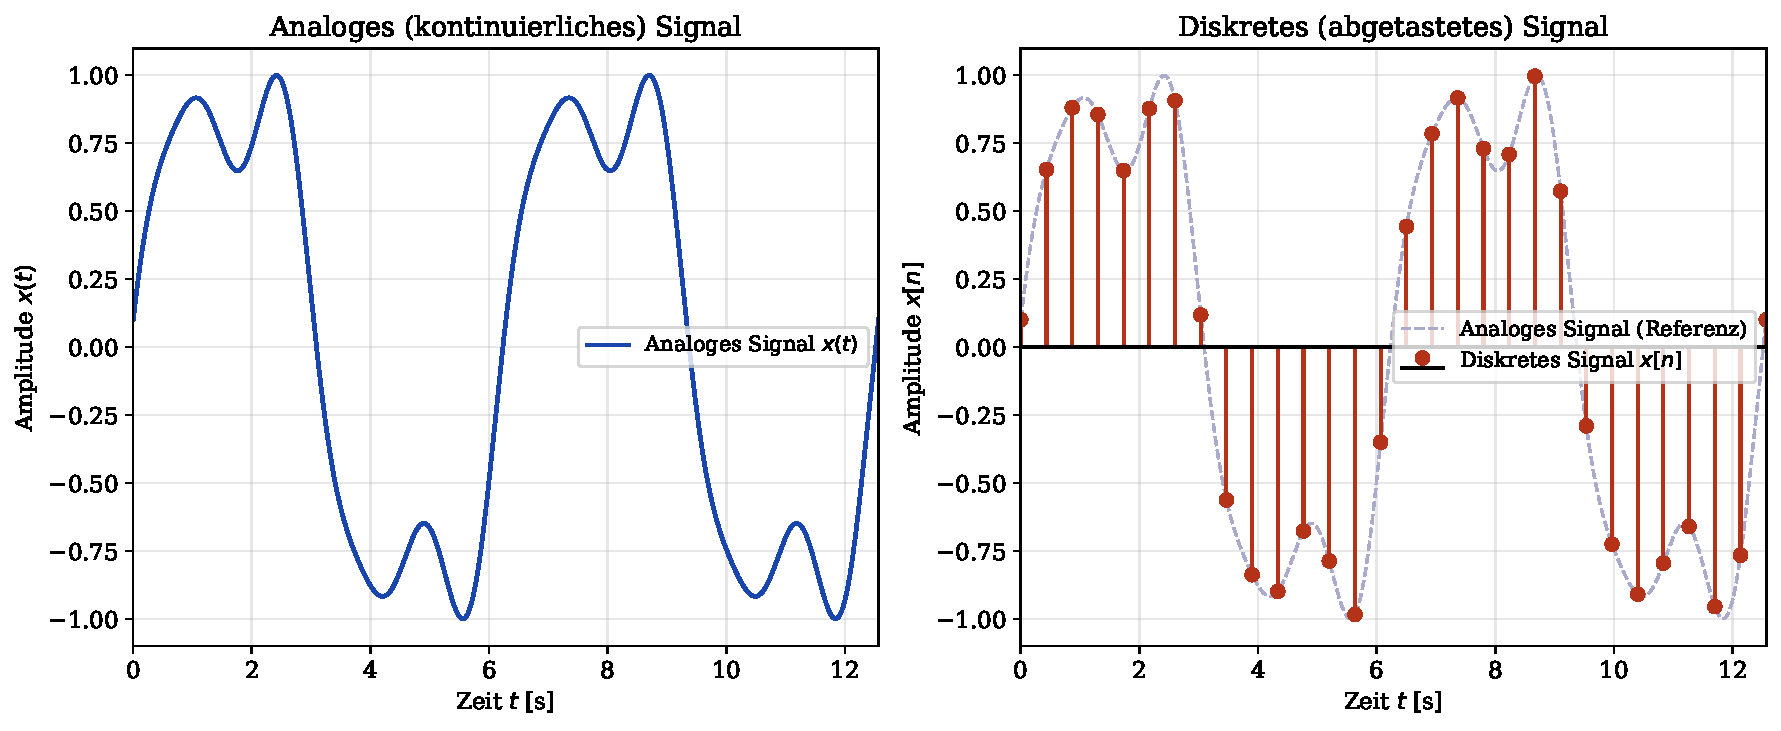
\includegraphics[width=\textwidth]{plot1_kontinuierlich_diskret.pdf}
    \caption{Vergleich eines analogen und eines diskreten Signals.
    \emph{Links:} Das analoge Signal $x(t) = \sin(t) + 0{,}3\sin(3t) + 0{,}1\cos(5t)$
    ist auf dem gesamten Intervall $[0, 4\pi]$ definiert und nimmt überabzählbar viele
    Zwischenwerte an.
    \emph{Rechts:} Das durch Abtastung mit 30 Stützstellen gewonnene diskrete Signal
    $x[n]$ verliert die kontinuierliche Information zwischen den Abtastzeitpunkten.
    Der Informationsverlust ist irreversibel, sofern die Bedingungen des
    Nyquist-Shannon-Theorems nicht erfüllt sind.}
    \label{fig:kontinuierlich}
\end{figure}

\begin{figure}[htbp]
    \centering
    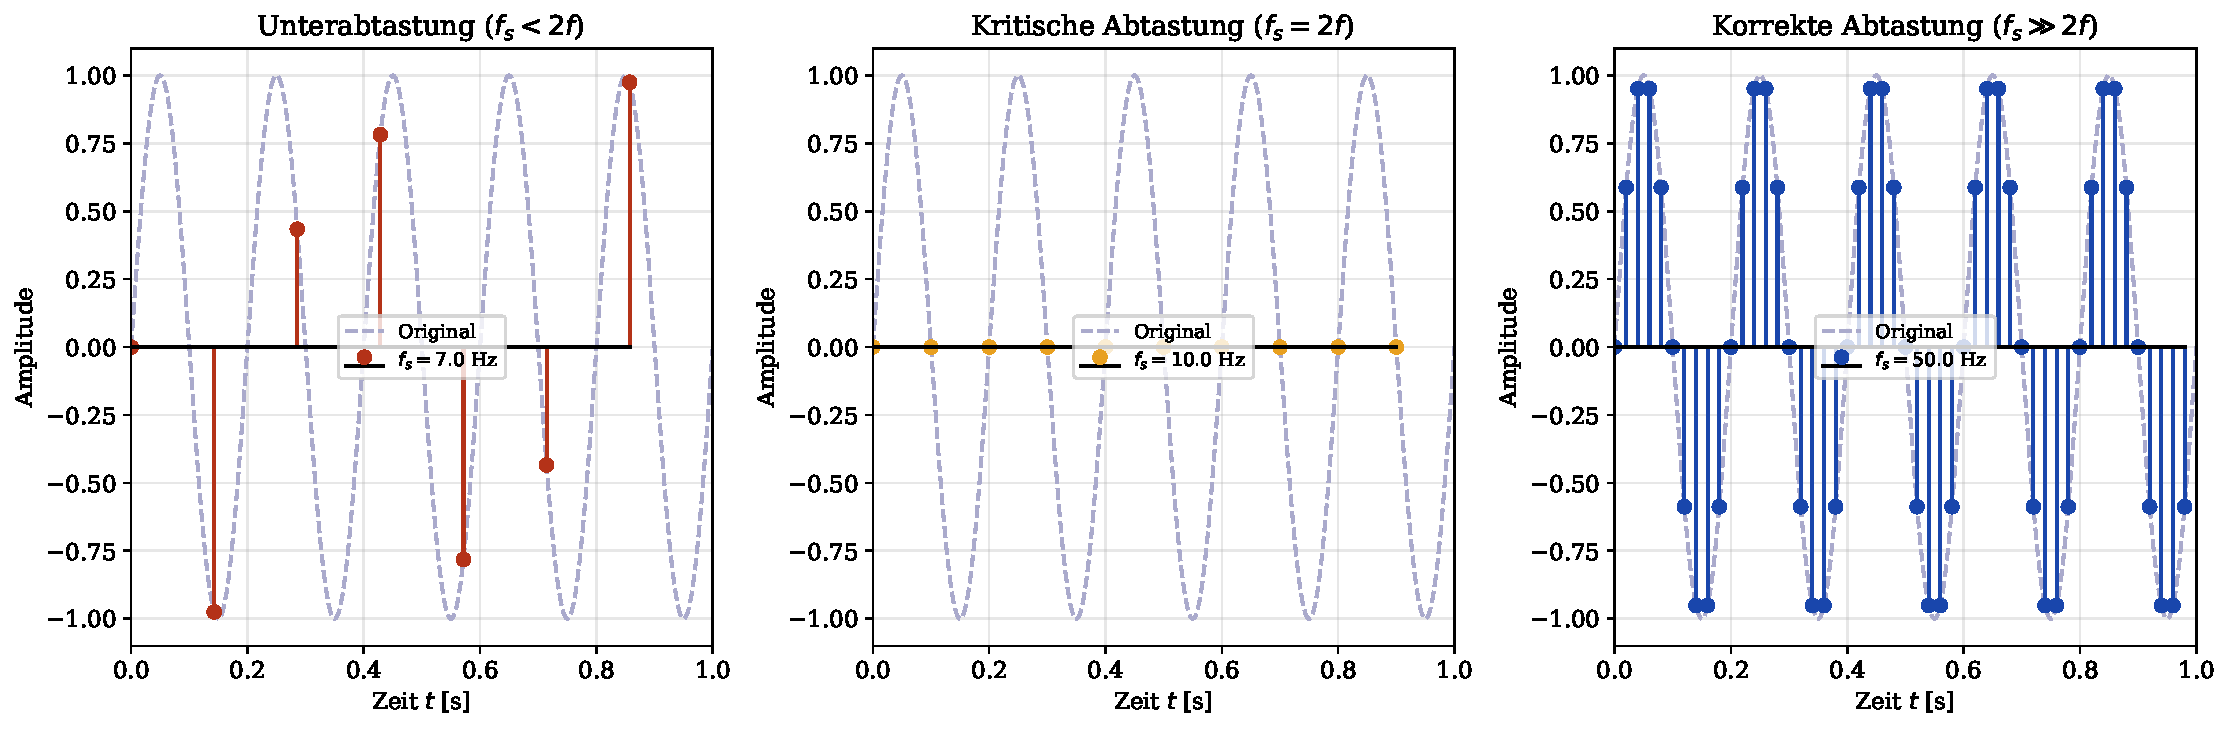
\includegraphics[width=\textwidth]{plot2_nyquist.pdf}
    \caption{Illustration des Nyquist-Shannon-Abtasttheorems (Satz~\ref{satz:nyquist})
    für ein Sinussignal der Frequenz $f = 5\,\mathrm{Hz}$.
    \emph{Links:} Bei Unterabtastung ($f_s = 7\,\mathrm{Hz} < 2 \cdot 5\,\mathrm{Hz}$)
    tritt Aliasing auf; das rekonstruierte Signal würde eine falsche Frequenz zeigen.
    \emph{Mitte:} An der Nyquist-Rate ($f_s = 10\,\mathrm{Hz}$) ist eine theoretisch
    perfekte, aber praktisch empfindliche Rekonstruktion möglich.
    \emph{Rechts:} Bei weit überkriterischer Abtastung ($f_s = 50\,\mathrm{Hz}$) ist
    die Hüllkurve des analogen Signals klar erkennbar.
    In jedem Fall bleibt das analoge Signal die primäre Entität; die Abtastwerte sind
    Messergebnisse einer diskreten Projektion.}
    \label{fig:nyquist}
\end{figure}

\begin{figure}[htbp]
    \centering
    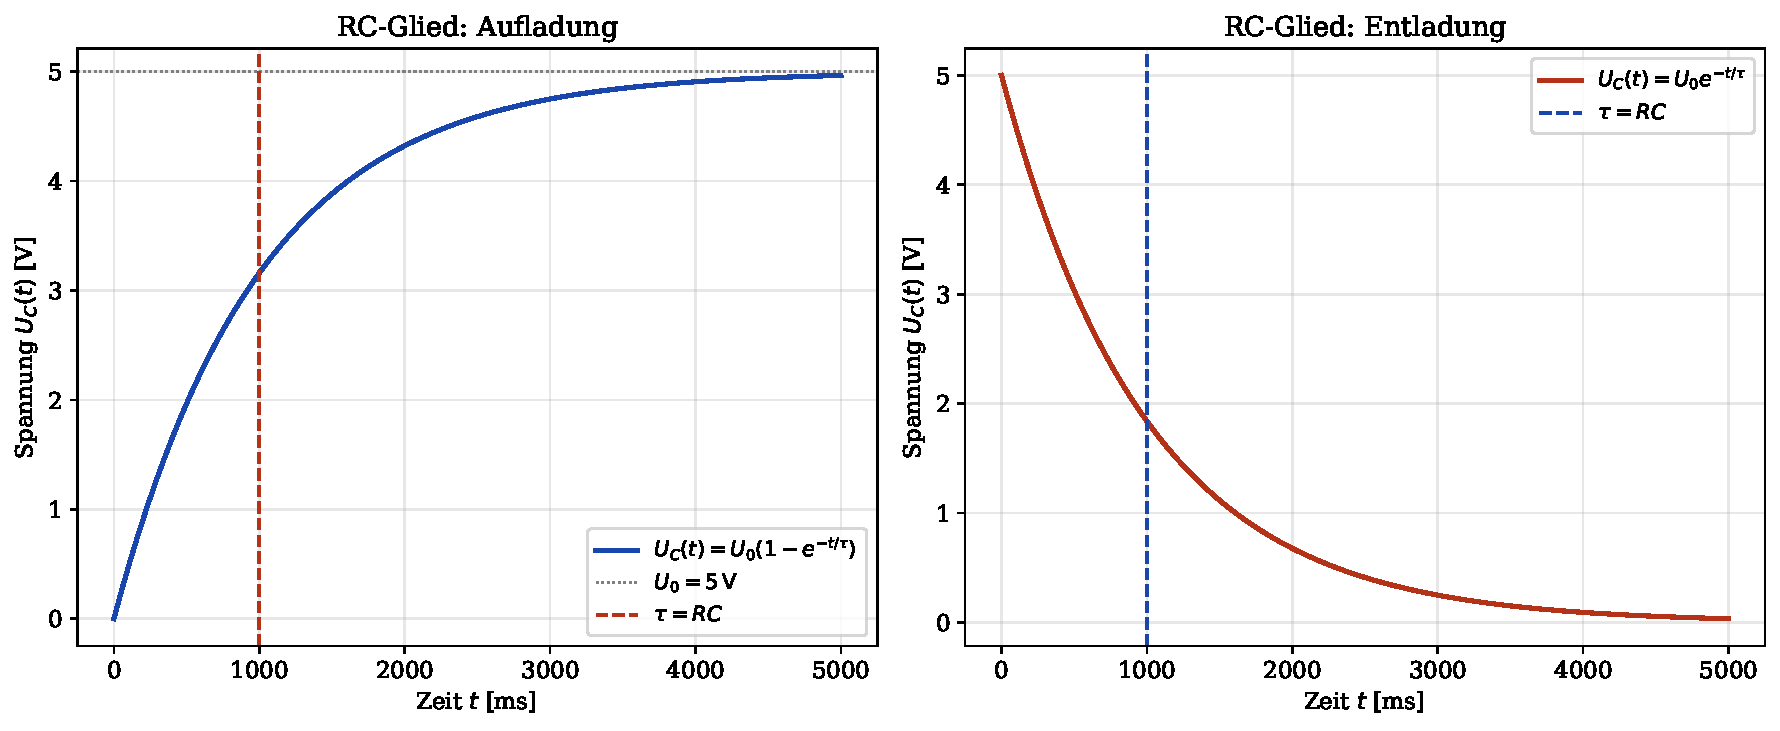
\includegraphics[width=\textwidth]{plot3_rc_glied.pdf}
    \caption{Lösung des RC-Glieds (Satz~\ref{satz:rc}) für $R = 1\,\mathrm{k\Omega}$,
    $C = 1\,\mathrm{mF}$, $\tau = RC = 1\,\mathrm{s}$, $U_0 = 5\,\mathrm{V}$.
    \emph{Links:} Aufladekurve $U_C(t) = U_0(1-e^{-t/\tau})$.  Die gestrichelte Linie
    markiert die Zeitkonstante $\tau$, bei der $U_C(\tau) = U_0(1-e^{-1}) \approx 3{,}16\,\mathrm{V}$.
    \emph{Rechts:} Entladekurve $U_C(t) = U_0 e^{-t/\tau}$.
    Beide Kurven sind transzendente Funktionen; ihre exakte Darstellung erfordert das
    reelle Kontinuum $\mathbb{R}$.}
    \label{fig:rc}
\end{figure}

\begin{figure}[htbp]
    \centering
    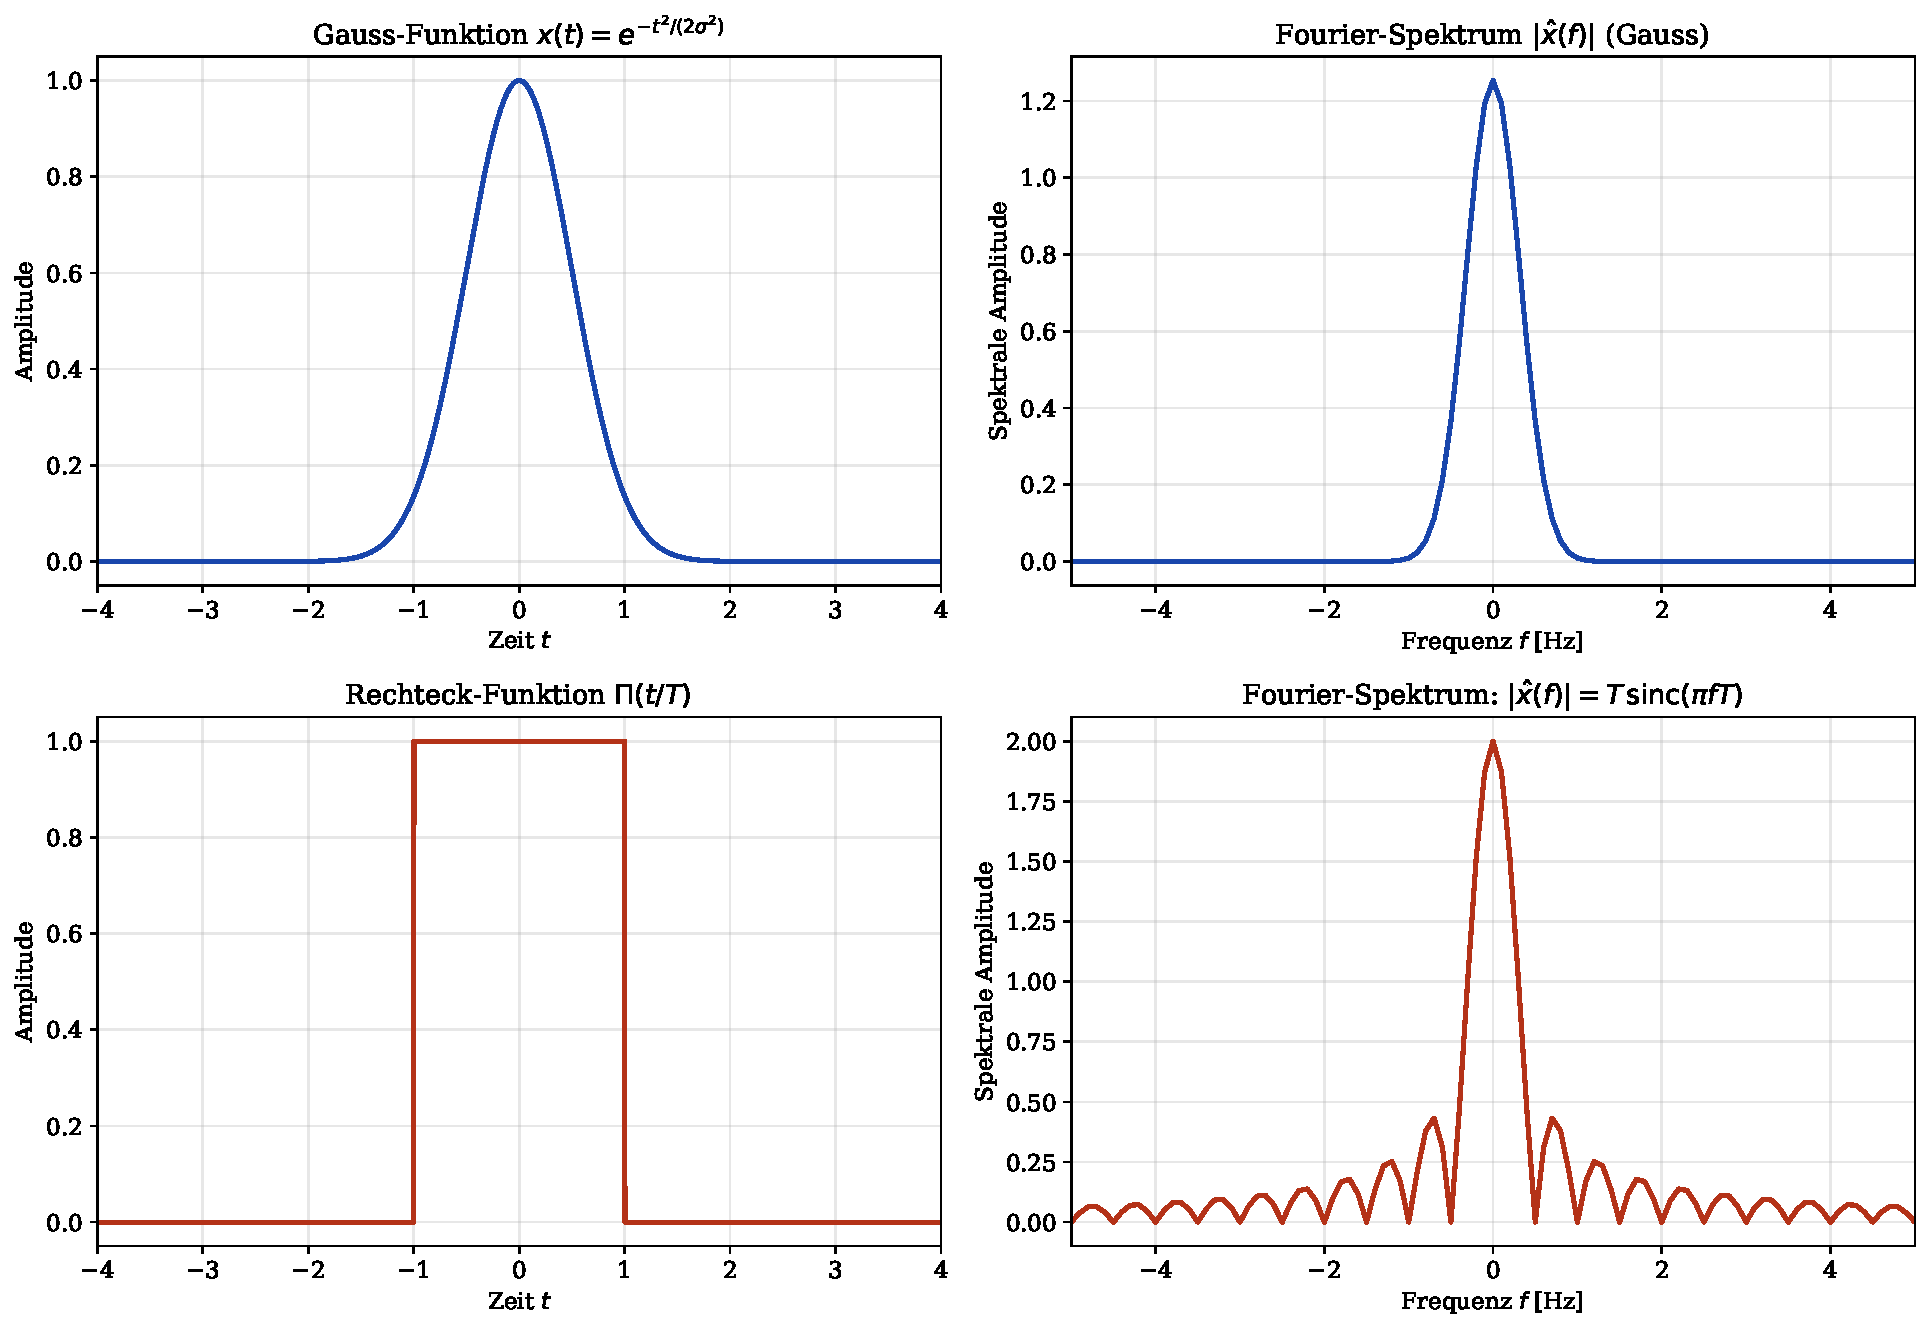
\includegraphics[width=\textwidth]{plot4_fourier.pdf}
    \caption{Fourier-Transformationspaare (Satz~\ref{satz:gauss}).
    \emph{Oben links/rechts:} Die Gauss-Funktion $x(t)=e^{-t^2/(2\sigma^2)}$ ist
    ein Eigenvektor der Fourier-Transformation; ihr Spektrum ist ebenfalls gaußförmig.
    Das Produkt $\Delta_t \cdot \Delta_f$ ist minimal und realisiert die
    Heisenberg-Schranke (Satz~\ref{satz:unschaerfe}).
    \emph{Unten links/rechts:} Die Rechteck-Funktion $\Pi(t/T)$ hat das Spektrum
    $|\hat{x}(f)| = T|\operatorname{sinc}(\pi fT)|$.  Die langsame Abklingrate des
    Sinc-Spektrums ($\sim 1/|f|$) illustriert die Unschärferelation: Ein
    zeitlich begrenztes Signal besitzt ein unendlich ausgedehntes Spektrum.}
    \label{fig:fourier}
\end{figure}

\begin{figure}[htbp]
    \centering
    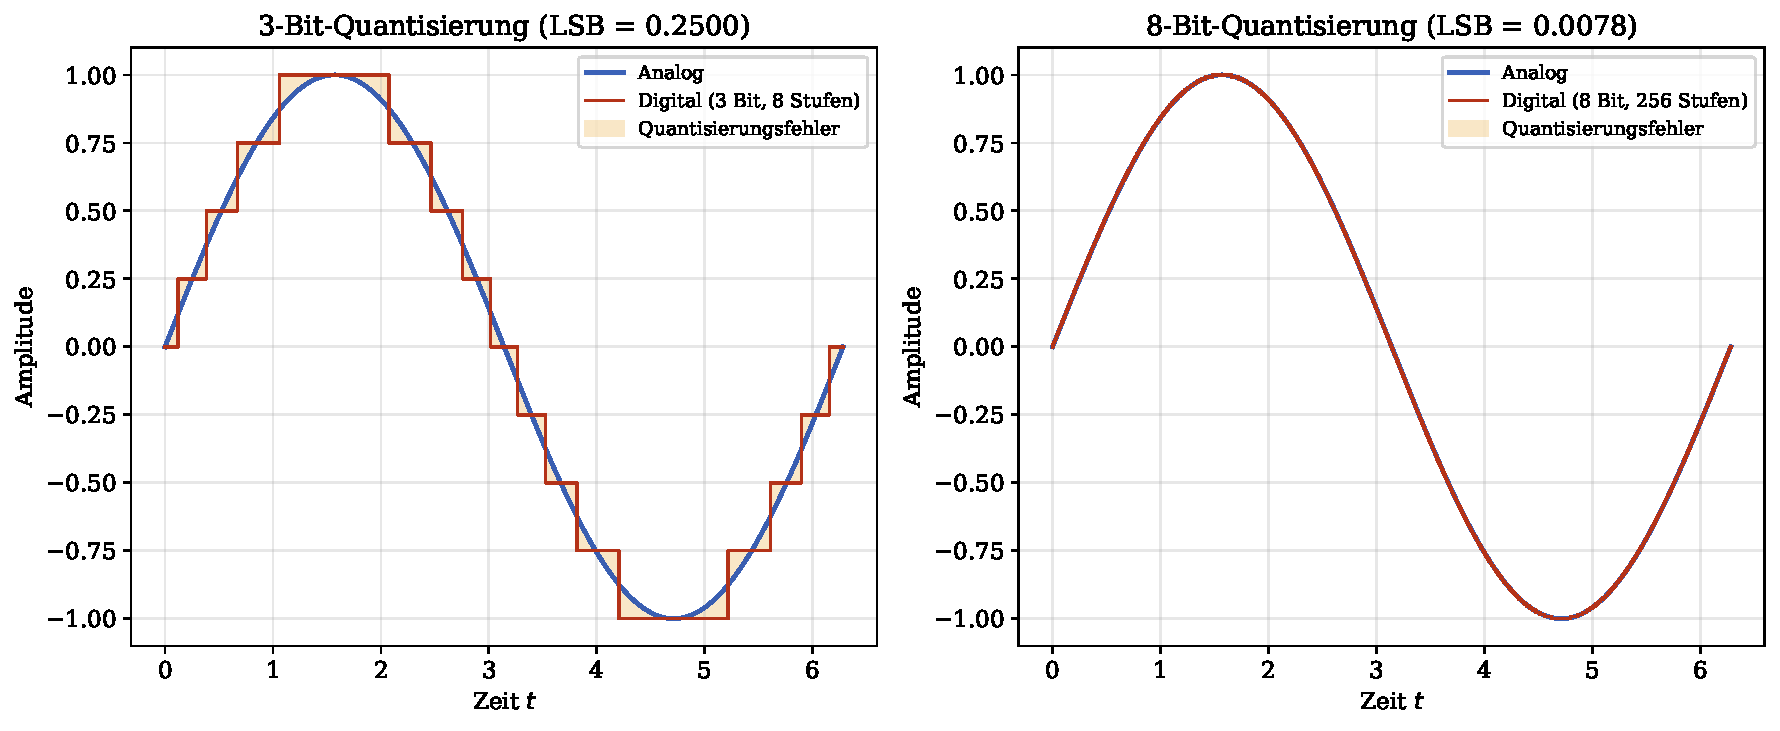
\includegraphics[width=\textwidth]{plot5_quantisierung.pdf}
    \caption{Quantisierungsfehler (Satz~\ref{satz:quantisierung}) bei 3~Bit
    ($\Delta = 0{,}25$) und 8~Bit ($\Delta \approx 0{,}0078$).
    Die orange Fläche zeigt den Quantisierungsfehler $e(t) = x(t) - Q_B(x(t))$.
    Bei 3~Bit ist der Fehler deutlich sichtbar;
    bei 8~Bit ist er stark reduziert, aber niemals null.
    Gemäß Satz~\ref{satz:quantisierung} beträgt das SQNR bei 3~Bit ca.~$19{,}8\,\mathrm{dB}$
    und bei 8~Bit ca.~$49{,}9\,\mathrm{dB}$.
    Die analoge Kurve bleibt in beiden Fällen die informationsreichste Darstellung.}
    \label{fig:quantisierung}
\end{figure}

\begin{figure}[htbp]
    \centering
    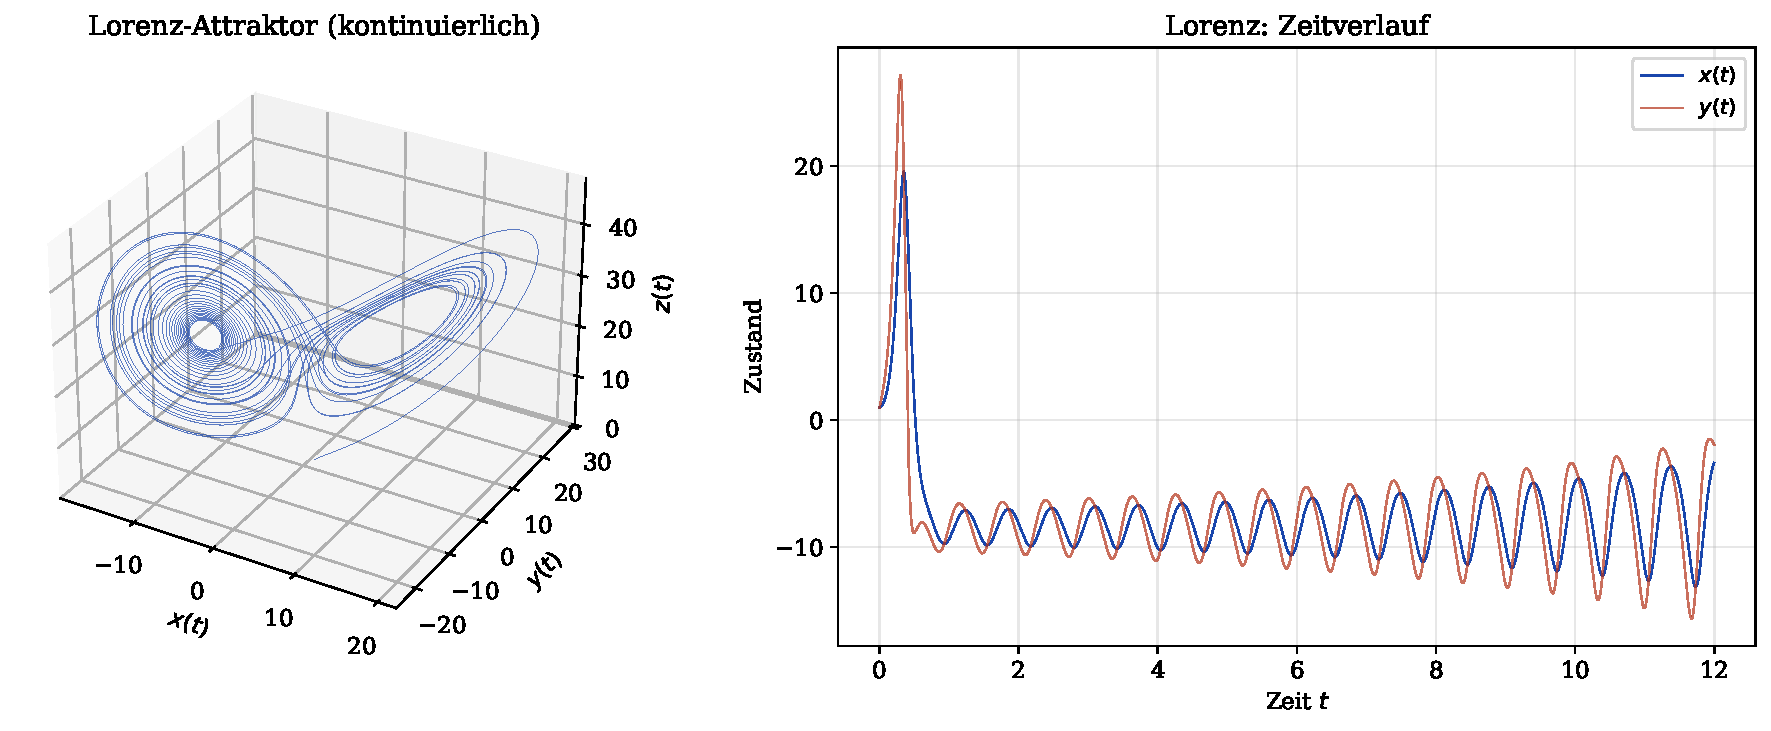
\includegraphics[width=\textwidth]{plot6_lorenz.pdf}
    \caption{Lorenz-Attraktor (Satz~\ref{satz:chaos}) für $\sigma=10$, $\rho=28$,
    $\beta=8/3$.
    \emph{Links:} Dreidimensionale Phasenraumtrajektorie über $t \in [0, 40]$.
    Die charakteristische Schmetterlingsform des seltsamen Attraktors zeigt die
    fraktale Struktur des Phasenraums.
    \emph{Rechts:} Zeitverlauf der Komponenten $x(t)$ und $y(t)$.
    Die sensitive Abhängigkeit von Anfangsbedingungen (positiver Lyapunov-Exponent
    $\lambda_{\max} \approx 0{,}905$) bedeutet, dass eine diskrete Simulation beliebig
    kleiner Genauigkeit das analoge Verhalten nur auf einer endlichen Zeitspanne
    korrekt wiedergibt.}
    \label{fig:lorenz}
\end{figure}

\begin{figure}[htbp]
    \centering
    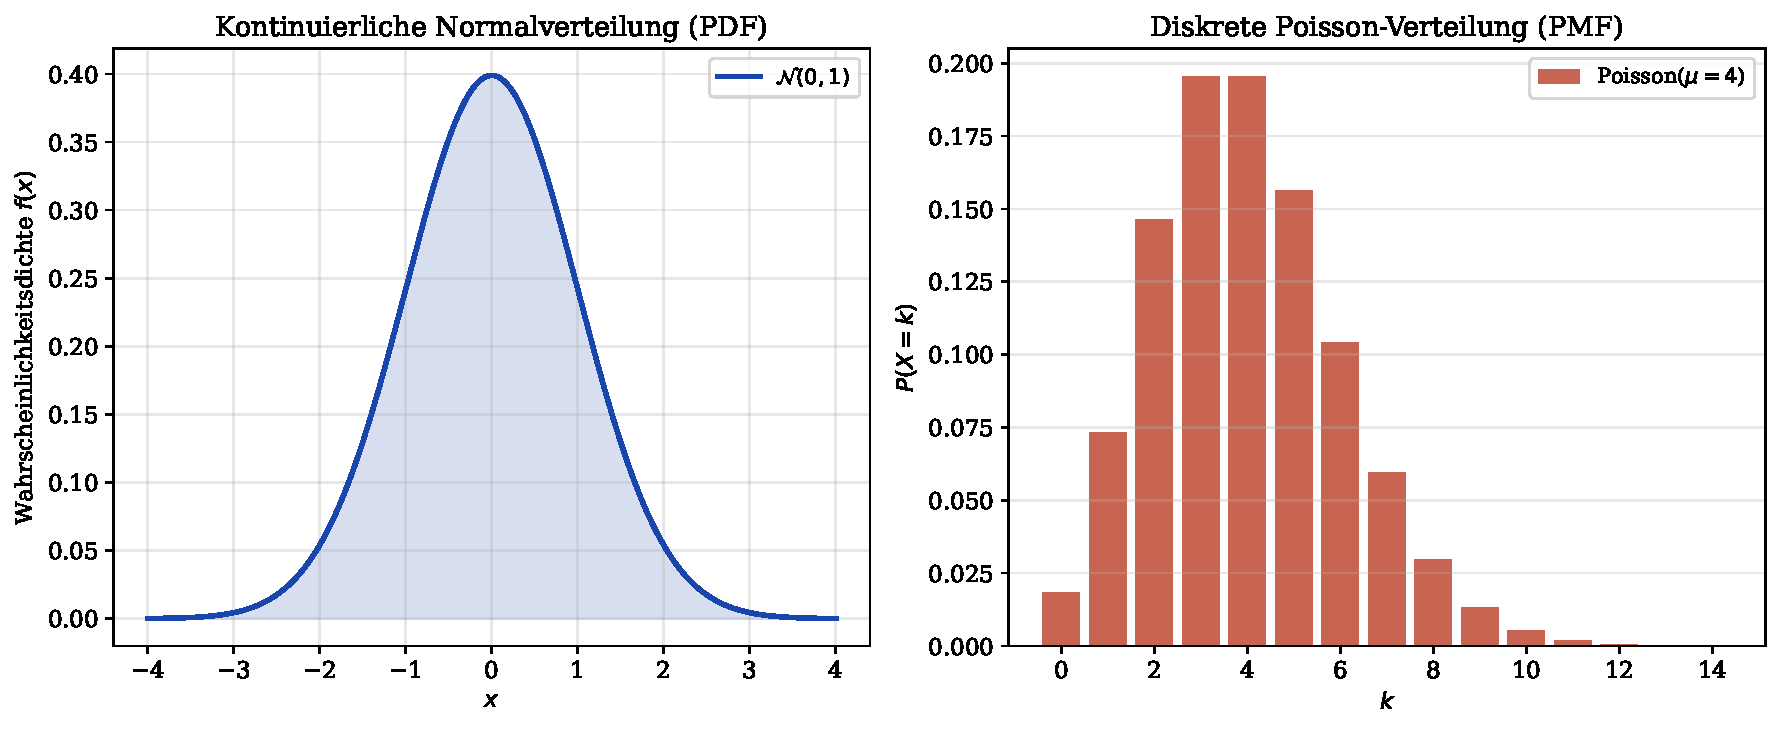
\includegraphics[width=\textwidth]{plot7_wahrscheinlichkeit.pdf}
    \caption{Kontinuierliche vs. diskrete Wahrscheinlichkeitsverteilungen.
    \emph{Links:} Die Normalverteilung $\mathcal{N}(0,1)$ ist eine Wahrscheinlichkeitsdichte
    (PDF) über $\mathbb{R}$.  Einzelne Punkte haben Wahrscheinlichkeit null;
    nur Intervalle $P(a \leq X \leq b) = \int_a^b f(x)dx$ sind sinnvoll.
    \emph{Rechts:} Die Poisson-Verteilung $\mathrm{Poi}(\mu=4)$ ist eine diskrete PMF.
    Die fundamentale Verschiedenheit beider Formalismen zeigt, dass kontinuierliche
    und diskrete Modelle verschiedene ontologische Ebenen beschreiben.}
    \label{fig:verteilungen}
\end{figure}

\begin{figure}[htbp]
    \centering
    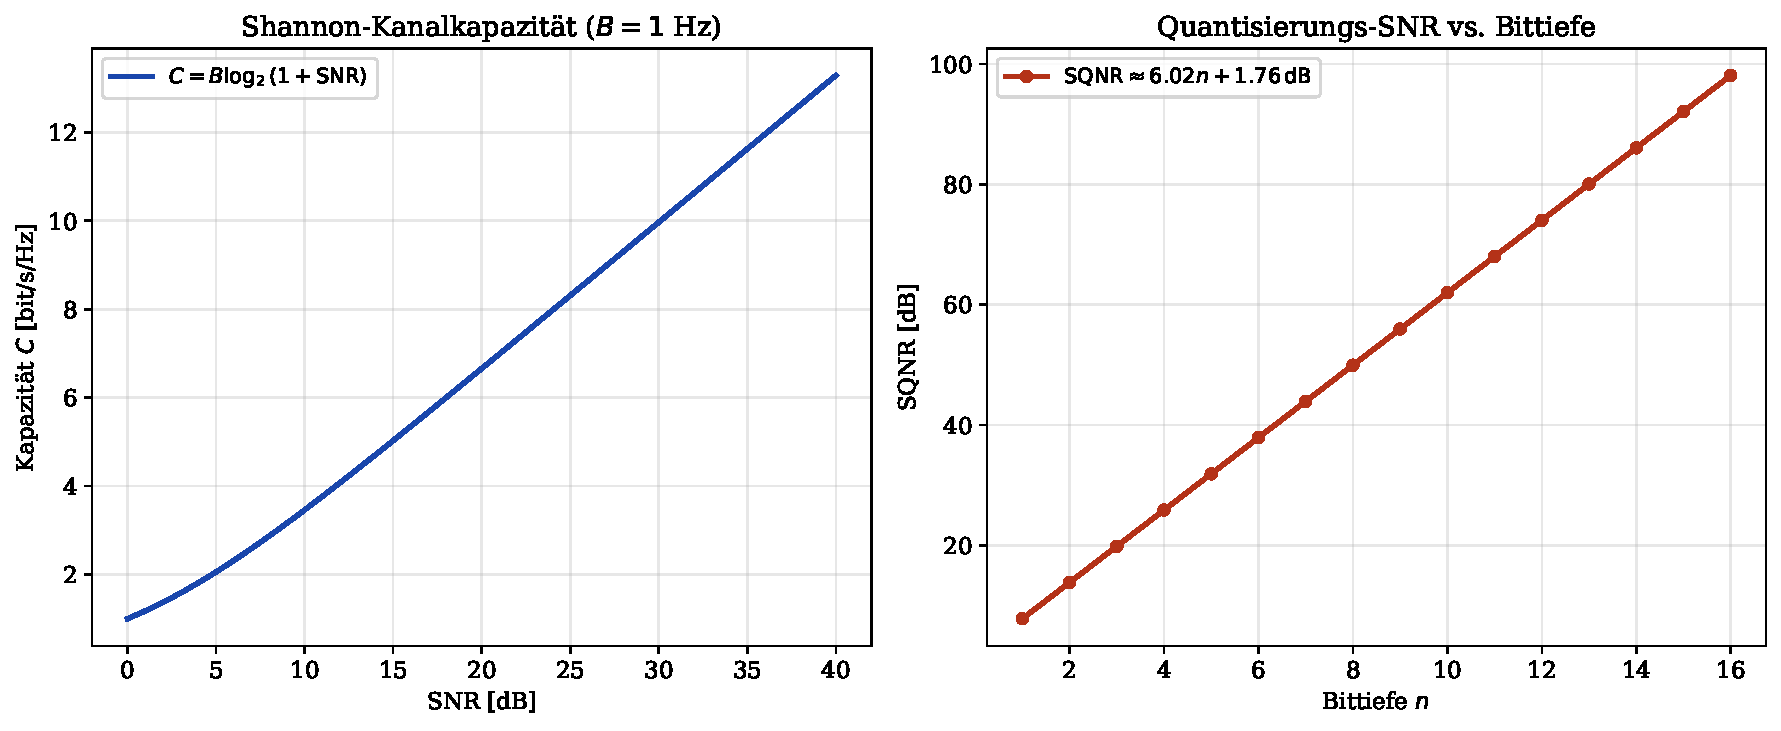
\includegraphics[width=\textwidth]{plot8_shannon.pdf}
    \caption{Informationstheoretische Grenzen.
    \emph{Links:} Shannon-Kanalkapazität $C = B\log_2(1+\mathrm{SNR})$
    (Satz~\ref{satz:shannon}) für $B = 1\,\mathrm{Hz}$ als Funktion des SNR.
    Die Kapazität wächst logarithmisch und ist unbegrenzt – eine Eigenschaft
    des analogen Kanals, nicht seiner digitalen Kodierung.
    \emph{Rechts:} SQNR als Funktion der Bittiefe $B$ nach der Faustformel
    $\mathrm{SQNR} \approx 6{,}02B + 1{,}76\,\mathrm{dB}$.
    Jedes zusätzliche Bit verbessert das SQNR um ca.~6~dB (Faktor 4 in der
    Leistung).  Dennoch bleibt für jede endliche Bittiefe ein Quantisierungsrestfehler.}
    \label{fig:shannon}
\end{figure}

% ===========================================================
\section{Zusammenfassung}
\label{sec:zusammenfassung}
% ===========================================================

Diese Arbeit hat formal nachgewiesen, dass \emph{Analog} nicht eine reaktive
Kategorie gegenüber dem Digitalen ist, sondern der ontologisch primäre Begriff
zur Beschreibung der physikalischen Realität.  Die zentralen Ergebnisse sind:

\begin{enumerate}
\item \textbf{Überabzählbarkeit} (Lemma~\ref{lem:ueberabzaehlbar}):
    Die reellen Zahlen sind überabzählbar; digitale Darstellungen können nur
    endlich oder abzählbar viele Werte repräsentieren.

\item \textbf{Hilbert-Raum-Struktur} (Satz~\ref{satz:vollstaendigkeit}):
    Analoge Signale bilden den vollständigen Hilbert-Raum $L^2(\mathbb{R})$;
    digitale Folgen bilden den abzählbaren Raum $\ell^2(\mathbb{Z})$.

\item \textbf{Fourier-Analysis} (Satz~\ref{satz:plancherel}):
    Die Fourier-Transformation ist eine unitäre Isometrie auf $L^2(\mathbb{R})$;
    die Energie-Erhaltung (Parseval) gilt exakt nur im Kontinuierlichen.

\item \textbf{Heisenberg-Unschärfe} (Satz~\ref{satz:unschaerfe}):
    $\Delta_t \cdot \Delta_f \geq 1/(4\pi)$ ist eine intrinsische Eigenschaft
    des analogen Signalraums, keine Messtechnologie.

\item \textbf{Physikalische Differenzialgleichungen}
    (Sätze~\ref{satz:picard},~\ref{satz:rc}):
    Alle fundamentalen Naturgesetze (Newton, Maxwell, Schrödinger) sind
    Differenzialgleichungen im Kontinuierlichen.

\item \textbf{Chaos und sensitive Abhängigkeit} (Satz~\ref{satz:chaos}):
    Chaotische Systeme zeigen, dass das Kontinuum nicht durch endliche digitale
    Genauigkeit langfristig approximiert werden kann.

\item \textbf{Nyquist-Shannon} (Satz~\ref{satz:nyquist}):
    Digitalisierung erfordert immer eine analoge Vorbedingung (Bandbreite);
    Aliasing bei Unterabtastung ist irreversibel.

\item \textbf{Quantisierungsrauschen} (Satz~\ref{satz:quantisierung}):
    Jede endliche Bittiefe erzeugt einen unvermeidlichen Informationsverlust.

\item \textbf{Shannon-Kapazität} (Satz~\ref{satz:shannon}):
    Die Kanalkapazität ist eine Eigenschaft des analogen Kanals;
    digitale Kodierung kann sie ausschöpfen, aber nicht übersteigen.
\end{enumerate}

% ===========================================================
\section{Ausblick}
\label{sec:ausblick}
% ===========================================================

Die in dieser Arbeit formal begründete Priorität des Analogen öffnet ein breites
Feld von Forschungsfragen, die im Folgenden systematisch und ausführlich dargelegt werden.

\subsection{Analoge Rechner und ihre Renaissance}

Die Dominanz digitaler Rechnerarchitekturen im 20. und frühen 21.~Jahrhundert hat
analoge Rechner weitgehend in die Nische gedrängt.  Doch in den letzten Jahren
erlebt die analoge Datenverarbeitung eine Renaissance, motiviert durch fundamentale
Einschränkungen der Silizium-CMOS-Technologie.

\subsubsection{Physikalische Grenzen digitaler CMOS-Technologie}

Mit zunehmender Miniaturisierung nähert sich die CMOS-Technologie physikalischen
Grenzen: Tunnelströme durch gate-oxide-Schichten der Stärke unter 1~nm,
Quanteneffekte in Transistorkanälen unter 5~nm Länge, und thermische Leistungsdichte-Grenzen
(„Power Wall'') bei ca.~100~W/cm² \citep{Taur1998}.  Diese Grenzen sind fundamental,
nicht ingenieurstechnisch.

\subsubsection{Neuromorphe Systeme als analoge Rechner}

Neuromorphe Chips wie Intel Loihi 2 und IBM TrueNorth implementieren
spiking neural networks, deren Grundoperationen inhärent analog sind:
Membranpotenziale, synaptische Gewichte und Schwellenwertmechanismen
operieren auf kontinuierlichen Größen, die durch analoge Schaltkreise
effizient realisiert werden \citep{Davies2021}.
Zukünftige Forschungsrichtungen umfassen:
\begin{itemize}
    \item Formale Spezifikationssprachen für analoge neuronale Netze
    \item Verifikation analoger Berechnungsmodelle durch differenzielle Spezifikation
    \item Hybride analog-digitale Architekturen mit optimaler Arbeitsaufteilung
    \item Energieeffizienz-Analyse mittels kontinuierlicher Optimierungstheorie
\end{itemize}

\subsubsection{Optische Analogrechner}

Optische Systeme führen Fourier-Transformationen physikalisch durch Lichtausbreitung
durch eine Linse aus – in $O(1)$ Zeit bezüglich der Signallänge.  Dies ist
algorithmisch schneller als jede digitale FFT.  Zukünftige Forschungsfelder sind:
\begin{itemize}
    \item Optische konvolutionelle neuronale Netze auf Basis der kontinuierlichen
          Fourier-Optik \citep{Lin2018}
    \item Diffractive Deep Neural Networks (D²NN) als analoge Lernarchitekturen
    \item Integration optischer Vorverarbeitung mit digitaler Nachverarbeitung
          (hybrid-photonische Computing-Systeme)
\end{itemize}

\subsection{Differenzialgleichungen als universelle Berechnungsmodelle}

\subsubsection{Turing-Vollständigkeit analoger Differenzialgleichungen}

Shannon \citep{Shannon1941} zeigte 1941, dass Analog-Differenzialrechner
(engl.\ \emph{general purpose analog computer}, GPAC) eine breite Klasse von
Funktionen berechnen können.  Die präzise Charakterisierung dieser Klasse –
die sog.\ \emph{differenzialgebraischen Funktionen} – gegenüber der Turing-Berechenbarkeit
ist ein aktives Forschungsfeld.

Offene Fragen:
\begin{itemize}
    \item Welche Klassen von Funktionen sind durch Differenzialgleichungen auf $\mathbb{R}$
          berechenbar, aber nicht durch Turing-Maschinen in polynomieller Zeit?
    \item Kann der Subgraph Algorithmus \citep{Epp2026subgraph} durch eine
          kontinuierliche Dynamik auf einem Attraktor implementiert werden?
    \item Wie verhält sich die analoge Berechnungskomplexität gegenüber der
          Beschreibungskomplexität von Differenzialgleichungssystemen?
\end{itemize}

\subsubsection{Neuronale gewöhnliche Differenzialgleichungen (Neural ODEs)}

Die 2018 eingeführten \emph{Neural Ordinary Differential Equations} (Neural ODEs)
\citep{Chen2018} interpretieren tiefe neuronale Netze als diskrete Approximationen
kontinuierlicher Flussfunktionen:
\[
\frac{d\mathbf{h}(t)}{dt} = f_\theta(\mathbf{h}(t), t).
\]
Dies zeigt, dass modernste maschinelle Lernmethoden selbst auf das Analoge
zurückgreifen, wenn Tiefe und Kontinuierlichkeit gemeinsam modelliert werden sollen.
Wichtige Forschungsrichtungen:
\begin{itemize}
    \item Stabilitätsanalyse lernbarer Differenzialgleichungssysteme
          (Lyapunov-Methoden für Neural ODEs)
    \item Kombination mit dem Subgraph Algorithmus zur Strukturerkennung
          in dynamischen Systemen \citep{Epp2026embedded}
    \item Zertifizierung und formale Verifikation von Neural ODEs nach
          ISO~26262 für sicherheitskritische eingebettete Systeme
\end{itemize}

\subsection{Analoge Signalverarbeitung und Messtechnik}

\subsubsection{Compressed Sensing und sparse Rekonstruktion}

Das Compressed-Sensing-Framework von Candès und Tao \citep{Candes2006}
zeigt, dass bandbegrenzte analoge Signale mit weniger als
Nyquist-vielen Messungen rekonstruierbar sind, sofern das Signal in einer
geeigneten Basis spärlich dargestellt werden kann:
\[
\mathbf{y} = \Phi \mathbf{x}, \quad \|\mathbf{x}\|_0 \ll N.
\]
Dies ist keine Widerlegung des Nyquist-Theorems, sondern eine Nutzung von
A-priori-Wissen über die Signalstruktur.  Wichtige offene Fragen:
\begin{itemize}
    \item Optimale analoge Messmatrizen $\Phi$ für kontinuierliche Signalklassen
    \item Rekonstruktionsgarantien bei analogen Rauschmodellen (nicht-Gaußsch)
    \item Robustheit gegenüber Modellfehlpassungen in der angenommenen Spärlichkeitsbasis
\end{itemize}

\subsubsection{Rauschen und stochastische Differenzialgleichungen}

Reale analoge Systeme sind stets verrauscht.  Das Rauschen wird durch
stochastische Differenzialgleichungen (Itô-Kalkül) beschrieben:
\[
d\mathbf{X}_t = \mu(\mathbf{X}_t, t) \, dt + \sigma(\mathbf{X}_t, t) \, d\mathbf{W}_t,
\]
wobei $\mathbf{W}_t$ ein Wiener-Prozess (Brownsche Bewegung) ist.
Zukünftige Forschung umfasst:
\begin{itemize}
    \item Filtertheorie für nichtlineare analoge Systeme (Kalman-Bucy-Filter
          und nichtlineare Erweiterungen)
    \item Stochastische Stabilitätsanalyse analoger neuronaler Netze
    \item Zusammenhang zwischen thermodynamischen Fluktuationen und analogem
          Informationsgehalt (Jarzynski-Gleichung, Landauer-Prinzip)
\end{itemize}

\subsection{Quantenmechanik als ultimative analoge Theorie}

\subsubsection{Die Schrödinger-Gleichung}

Die quantenmechanische Wellenfunktion $\Psi: \mathbb{R}^3 \times \mathbb{R} \to \mathbb{C}$
genügt der zeitabhängigen Schrödinger-Gleichung:
\[
i\hbar \frac{\partial \Psi}{\partial t} = \hat{H} \Psi,
\]
wobei $\hat{H}$ der Hamilton-Operator ist.  Die Wellenfunktion ist eine
kontinuierliche, komplexwertige Funktion im Hilbert-Raum $L^2(\mathbb{R}^3)$.
Die Messung erzeugt Quantisierung (diskrete Eigenwerte), aber die Dynamik
zwischen Messungen ist fundamental kontinuierlich.

\subsubsection{Quantenfeldtheorie und das Pfadintegral}

Im Rahmen der Quantenfeldtheorie (QFT) werden Ãœbergangsamplituden als
Pfadintegrale über den gesamten Raum aller kontinuierlichen Feldkonfigurationen
berechnet:
\[
\langle \phi_f | e^{-iHT/\hbar} | \phi_i \rangle
= \int_{\phi(0)=\phi_i}^{\phi(T)=\phi_f} \mathcal{D}\phi \; e^{iS[\phi]/\hbar},
\]
wobei $S[\phi]$ die Wirkung ist.  Dieses Pfadintegral ist buchstäblich eine
Integration über überabzählbar viele kontinuierliche Pfade \citep{Feynman1965}.
Dies zeigt: Die fundamentalste Theorie der Materie ist analog.

\subsubsection{Analog-Quanten-Computing}

Analoge Quantensimulatoren (z.\,B.\ mit ultrakalten Atomen) implementieren
Quantenmodelle durch kontinuierliche Kontrolle von Laser- und Magnetfeldparametern.
Im Gegensatz zu gate-basierten Quantencomputern arbeiten sie im analogen Regime
und können natürliche Quantenphänomene effizienter simulieren \citep{Bloch2012}.

\subsection{Philosophische und wissenschaftstheoretische Implikationen}

\subsubsection{Kontinuierliche Ontologie vs. diskrete Darstellung}

Die in dieser Arbeit formal entwickelte Unterscheidung zwischen
\emph{ontologischer Kontinuierlichkeit} (die Welt ist analog) und
\emph{epistemischer Diskretheit} (wir messen und speichern digital) hat
tiefe wissenschaftstheoretische Konsequenzen.  Physikalische Gesetze werden
in der Sprache des Kontinuums formuliert; ihre Überprüfung erfordert immer
den Rückbezug auf das Analoge als Maßstab.

\subsubsection{Das Messproblem}

Jede Messung einer physikalischen Größe ist eine Projektion des
analogen Kontinuums auf eine diskrete oder endlich genaue Zahl.
Das Messproblem der Quantenmechanik ist in diesem Sinne ein besonderer Fall
des allgemeinen Problems, wie diskrete Beobachtungen aus einer kontinuierlichen
Dynamik entstehen.

\subsubsection{Leibniz vs. Newton: Das Kontinuum als Basis}

Die historische Debatte zwischen Leibniz und Newton über das Kontinuum und den
Infinitesimalkalkül \citep{Leibniz1684} hat eine zeitlose Relevanz:
Die Differenzialrechnung als Sprache der Naturgesetze setzt das Kontinuum voraus.
Jeder Versuch, die Natur fundamental digital zu beschreiben (digitale Physik,
cellular automata als Weltmodell nach Wolfram \citep{Wolfram2002}), stößt auf
das Problem, kontinuierliche Symmetrien (Translationsinvarianz, Lorentz-Invarianz)
in einem diskreten Gitter zu implementieren.

\subsection{Ingenieurstechnische Implikationen für eingebettete Systeme}

\subsubsection{AUTOSAR und analoge Sensorsignalverarbeitung}

In modernen Kraftfahrzeugen werden analoge Sensor-Signale (Beschleunigung,
Druck, Temperatur, Strom) durch AUTOSAR-konforme Software-Komponenten
verarbeitet.  Die korrekte Modellierung der analogen Signalkette
(Sensor $\to$ ADC $\to$ Signal Conditioning $\to$ Algorithmus) erfordert
formale Methoden zur Fehleranalyse \citep{Autosar2023}:
\begin{itemize}
    \item Formale Spezifikation analoger Sensorbandbreiten in AUTOSAR-Schnittstellen
    \item Nachweis, dass digitale Algorithmen die analogen Anforderungen nach
          ISO~26262 erfüllen (ASIL-Klassifikation)
    \item Anwendung des Subgraph Algorithmus \citep{Epp2026embedded} zur
          strukturellen Überprüfung von Signalverarbeitungsgraphen
\end{itemize}

\subsubsection{EtherCAT und Echtzeitfähigkeit}

EtherCAT-Systeme kommunizieren mit Zykluszeiten im Mikrosekundenbereich,
die an die Nyquist-Rate der angebundenen analogen Prozesse angepasst werden müssen.
Der formale Nachweis der Abtastraten-Konformität ist ein offenes Problem der
eingebetteten Systementwicklung \citep{Epp2026ehae}.

\subsubsection{Regelungstechnik: Kontinuierliche vs. diskrete Regler}

In der Regelungstechnik werden kontinuierliche Systemmodelle
(Ãœbertragungsfunktionen, Zustandsraumdarstellungen) durch diskrete
Implementierungen (z-Transformation, Euler-Diskretisierung) approximiert.
Die Güte dieser Approximation hängt vom Verhältnis der Abtastrate zur
Systembandbreite ab und ist Gegenstand aktiver Forschung:
\begin{itemize}
    \item Entwurf von Reglern, die explizit die analoge Systemnatur berücksichtigen
          (sampled-data control theory)
    \item Robustheit diskreter Regler bei analogen Modellfehlern
    \item Implementierung auf MicroPython/ESP32 (PyLab-Framework \citep{Epp2026pylab})
          mit präziser Zeitsteuerung
\end{itemize}

\subsection{Weiterführende mathematische Fragen}

\subsubsection{Wavelet-Analysis als lokale Fourier-Theorie}

Während die Fourier-Transformation das globale Spektrum eines analogen Signals
erfasst, erlaubt die Wavelet-Transformation eine simultane Zeit-Frequenz-Lokalisierung:
\[
(Wf)(a,b) = \frac{1}{\sqrt{a}} \int_{-\infty}^\infty f(t) \, \overline{\psi\!\left(\frac{t-b}{a}\right)} \, dt,
\]
wobei $\psi$ das Mutter-Wavelet ist.  Offene Forschungsfragen:
\begin{itemize}
    \item Optimale Wavelet-Basen für spezifische physikalische Signalklassen
    \item Verbindung zur fraktalen Geometrie chaotischer Attraktoren
    \item Kontinuierliche Wavelet-Transformationen auf Lie-Gruppen
          als Verallgemeinerung für mehrdimensionale analoge Signale
\end{itemize}

\subsubsection{Nicht-Standardanalyse und Infinitesimale}

Die Non-Standard-Analysis nach Abraham Robinson \citep{Robinson1966} bietet
einen streng mathematischen Rahmen für Infinitesimale, der die intuitive
Vorstellung des Kontinuums als aus ``unendlich kleinen'' Teilen bestehend
formalisiert.  Eine formalere Verbindung zwischen:
\begin{itemize}
    \item Non-Standard-Analysis und analoger Signalverarbeitung
    \item Infinitesimalen Größen und physikalischen Messgenauigkeitsgrenzen
    \item Hyperreellen Zahlen ${}^*\mathbb{R}$ als Modell physikalischer Messgrößen
\end{itemize}
steht als offenes Forschungsgebiet bereit.

\subsubsection{Topos-Theorie und kontinuierliche Logik}

Die kategorientheoretische Topos-Theorie \citep{Lawvere1968} erlaubt die
Formulierung von Logik über allgemeinen topologischen Räumen und damit die
Untersuchung von Aussagen, deren Wahrheitswerte kontinuierlich variieren
(Fuzzy-Logik als Spezialfall).  Physikalische Modelle mit kontinuierlichen
Parametern könnten in diesem Rahmen präziser spezifiziert werden als
durch klassische binäre Logik.

\subsection{Zusammenfassung des Ausblicks}

Die ontologische Priorität des Analogen eröffnet eine Fülle von Forschungsrichtungen:
von der Renaissance analoger Rechnerarchitekturen über Neural ODEs und
Quantencomputing bis zu fundamentalen Fragen der Wissenschaftsphilosophie
und formaler Verifikation eingebetteter Systeme.  Gemeinsam ist diesen Richtungen,
dass sie das Digitale nicht als Ersatz des Analogen verstehen, sondern als
eine Projektion oder Näherung, die immer auf den reichen Informationsgehalt
des Kontinuums zurückverweist.

Das Programm einer vollständigen formalen Grundlegung der analogen
Signalverarbeitung – verbunden mit Anwendungen in eingebetteten Systemen,
quantenmechanischen Modellen und neuronalen Differenzialgleichungen –
bleibt ein offenes, produktives und fundamental wichtiges Forschungsfeld.
Der Autor wird diese Fragen in nachfolgenden Arbeiten \citep{Epp2026analog}
weiter vertiefen.

% ===========================================================
\bibliographystyle{plainnat}
\bibliography{analog}
% ===========================================================

\end{document}

